\documentclass[journal,12pt,twocolumn]{IEEEtran}
\hbadness = 10001
\vbadness = 10001
\usepackage{setspace}
\usepackage{textcomp}
\usepackage{gensymb}
\usepackage{xcolor}
\usepackage{caption}
%\usepackage{subcaption}
%\doublespacing
\singlespacing
%\usepackage{graphicx}
%\usepackage{amssymb}
%\usepackage{relsize}
\usepackage[cmex10]{amsmath}
\usepackage{mathtools}
%\usepackage{amsthm}
%\interdisplaylinepenalty=2500
%\savesymbol{iint}
%\usepackage{txfonts}
%\restoresymbol{TXF}{iint}
%\usepackage{wasysym}
\usepackage{hyperref}
\usepackage{amsthm}
\usepackage{mathrsfs}
\usepackage{txfonts}
\usepackage{stfloats}
\usepackage{cite}
\usepackage{cases}
\usepackage{subfig}
%\usepackage{xtab}
\usepackage{longtable}
\usepackage{multirow}
%\usepackage{algorithm}
%\usepackage{algpseudocode}
%\usepackage{enumerate}
\usepackage{enumitem}
\usepackage{mathtools}
%\usepackage{iithtlc}
%\usepackage[framemethod=tikz]{mdframed}
\usepackage{xfrac}
\usepackage{listings}
\usepackage{tikz}
\usetikzlibrary{shapes,arrows,positioning}
\usepackage[RPvoltages]{circuitikz}
\let\vec\mathbf


%\usepackage{stmaryrd}

%\usepackage{wasysym}
%\newcounter{MYtempeqncnt}
\DeclareMathOperator*{\Res}{Res}
%\renewcommand{\baselinestretch}{2}
\renewcommand\thesection{\arabic{section}}
\renewcommand\thesubsection{\thesection.\arabic{subsection}}
\renewcommand\thesubsubsection{\thesubsection.\arabic{subsubsection}}

\renewcommand\thesectiondis{\arabic{section}}
\renewcommand\thesubsectiondis{\thesectiondis.\arabic{subsection}}
\renewcommand\thesubsubsectiondis{\thesubsectiondis.\arabic{subsubsection}}

%\renewcommand{\labelenumi}{\textbf{\theenumi}}
%\renewcommand{\theenumi}{P.\arabic{enumi}}

% correct bad hyphenation here
\hyphenation{op-tical net-works semi-conduc-tor}

\lstset{
language=Python,
frame=single, 
breaklines=true,
columns=fullflexible
}



\begin{document}
%

\theoremstyle{definition}
\newtheorem{theorem}{Theorem}[section]
\newtheorem{problem}{Problem}
\newtheorem{proposition}{Proposition}[section]
\newtheorem{lemma}{Lemma}[section]
\newtheorem{corollary}[theorem]{Corollary}
\newtheorem{example}{Example}[section]
\newtheorem{definition}{Definition}[section]
%\newtheorem{algorithm}{Algorithm}[section]
%\newtheorem{cor}{Corollary}
\newcommand{\BEQA}{\begin{eqnarray}}
\newcommand{\EEQA}{\end{eqnarray}}
\newcommand{\define}{\stackrel{\triangle}{=}}
\newcommand{\myvec}[1]{\ensuremath{\begin{pmatrix}#1\end{pmatrix}}}
\newcommand{\mydet}[1]{\ensuremath{\begin{vmatrix}#1\end{vmatrix}}}

\bibliographystyle{IEEEtran}
%\bibliographystyle{ieeetr}

\providecommand{\nCr}[2]{\,^{#1}C_{#2}} % nCr
\providecommand{\nPr}[2]{\,^{#1}P_{#2}} % nPr
\providecommand{\mbf}{\mathbf}
\providecommand{\pr}[1]{\ensuremath{\Pr\left(#1\right)}}
\providecommand{\qfunc}[1]{\ensuremath{Q\left(#1\right)}}
\providecommand{\sbrak}[1]{\ensuremath{{}\left[#1\right]}}
\providecommand{\lsbrak}[1]{\ensuremath{{}\left[#1\right.}}
\providecommand{\rsbrak}[1]{\ensuremath{{}\left.#1\right]}}
\providecommand{\brak}[1]{\ensuremath{\left(#1\right)}}
\providecommand{\lbrak}[1]{\ensuremath{\left(#1\right.}}
\providecommand{\rbrak}[1]{\ensuremath{\left.#1\right)}}
\providecommand{\cbrak}[1]{\ensuremath{\left\{#1\right\}}}
\providecommand{\lcbrak}[1]{\ensuremath{\left\{#1\right.}}
\providecommand{\rcbrak}[1]{\ensuremath{\left.#1\right\}}}
\theoremstyle{remark}
\newtheorem{rem}{Remark}
\newcommand{\sgn}{\mathop{\mathrm{sgn}}}
\providecommand{\abs}[1]{\left\vert#1\right\vert}
\providecommand{\res}[1]{\Res\displaylimits_{#1}} 
\providecommand{\norm}[1]{\lVert#1\rVert}
\providecommand{\mtx}[1]{\mathbf{#1}}
\providecommand{\mean}[1]{E\left[ #1 \right]}
\providecommand{\fourier}{\overset{\mathcal{F}}{ \rightleftharpoons}}
\providecommand{\ztrans}{\overset{\mathcal{Z}}{ \rightleftharpoons}}

%\providecommand{\hilbert}{\overset{\mathcal{H}}{ \rightleftharpoons}}
\providecommand{\system}{\overset{\mathcal{H}}{ \longleftrightarrow}}
%\newcommand{\solution}[2]{\textbf{Solution:}{#1}}
\newcommand{\solution}{\noindent \textbf{Solution: }}
\providecommand{\dec}[2]{\ensuremath{\overset{#1}{\underset{#2}{\gtrless}}}}
\numberwithin{equation}{section}
%\numberwithin{equation}{subsection}
%\numberwithin{problem}{subsection}
%\numberwithin{definition}{subsection}
\makeatletter
\@addtoreset{figure}{problem}
\makeatother

\let\StandardTheFigure\thefigure
%\renewcommand{\thefigure}{\theproblem.\arabic{figure}}
\renewcommand{\thefigure}{\theproblem}


%\numberwithin{figure}{subsection}

\def\putbox#1#2#3{\makebox[0in][l]{\makebox[#1][l]{}\raisebox{\baselineskip}[0in][0in]{\raisebox{#2}[0in][0in]{#3}}}}
\def\rightbox#1{\makebox[0in][r]{#1}}
\def\centbox#1{\makebox[0in]{#1}}
\def\topbox#1{\raisebox{-\baselineskip}[0in][0in]{#1}}
\def\midbox#1{\raisebox{-0.5\baselineskip}[0in][0in]{#1}}

\vspace{3cm}

\title{ 
%\logo{
%}
Circuits and Transforms
%	\logo{Octave for Math Computing }
}
%\title{
%	\logo{Matrix Analysis through Octave}{\begin{center}\includegraphics[scale=.24]{tlc}\end{center}}{}{HAMDSP}
%}


% paper title
% can use linebreaks \\ within to get better formatting as desired
%\title{Matrix Analysis through Octave}
%
%
% author names and IEEE memberships
% note positions of commas and nonbreaking spaces ( ~ ) LaTeX will not break
% a structure at a ~ so this keeps an author's name from being broken across
% two lines.
% use \thanks{} to gain access to the first footnote area
% a separate \thanks must be used for each paragraph as LaTeX2e's \thanks
% was not built to handle multiple paragraphs
%

\author{ G V V Sharma$^{*}$ %<-this  stops a space
\thanks{*The author is with the Department
of Electrical Engineering, Indian Institute of Technology, Hyderabad
502285 India e-mail:  gadepall@iith.ac.in.  All content in the manuscript is 
released under GNU GPL.  Free to use for anything. }% <-this % stops a space
%\thanks{J. Doe and J. Doe are with Anonymous University.}% <-this % stops a space
%\thanks{Manuscript received April 19, 2005; revised January 11, 2007.}}
}
% note the % following the last \IEEEmembership and also \thanks - 
% these prevent an unwanted space from occurring between the last author name
% and the end of the author line. i.e., if you had this:
% 
% \author{....lastname \thanks{...} \thanks{...} }
%                     ^------------^------------^----Do not want these spaces!
%
% a space would be appended to the last name and could cause every name on that
% line to be shifted left slightly. This is one of those "LaTeX things". For
% instance, "\textbf{A} \textbf{B}" will typeset as "A B" not "AB". To get
% "AB" then you have to do: "\textbf{A}\textbf{B}"
% \thanks is no different in this regard, so shield the last } of each \thanks
% that ends a line with a % and do not let a space in before the next \thanks.
% Spaces after \IEEEmembership other than the last one are OK (and needed) as
% you are supposed to have spaces between the names. For what it is worth,
% this is a minor point as most people would not even notice if the said evil
% space somehow managed to creep in.



% The paper headers
%\markboth{Journal of \LaTeX\ Class Files,~Vol.~6, No.~1, January~2007}%
%{Shell \MakeLowercase{\textit{et al.}}: Bare Demo of IEEEtran.cls for Journals}
% The only time the second header will appear is for the odd numbered pages
% after the title page when using the twoside option.
% 
% *** Note that you probably will NOT want to include the author's ***
% *** name in the headers of peer review papers.                   ***
% You can use \ifCLASSOPTIONpeerreview for conditional compilation here if
% you desire.




% If you want to put a publisher's ID mark on the page you can do it like
% this:
%\IEEEpubid{0000--0000/00\$00.00~\copyright~2007 IEEE}
% Remember, if you use this you must call \IEEEpubidadjcol in the second
% column for its text to clear the IEEEpubid mark.



% make the title area
\maketitle

%\newpage

%\renewcommand{\thefigure}{\thesection.\theenumi}
%\renewcommand{\thetable}{\thesection.\theenumi}

\renewcommand{\thefigure}{\theenumi}
\renewcommand{\thetable}{\theenumi}

%\renewcommand{\theequation}{\thesection}


\bigskip

\begin{abstract}
This manual provides a simple introduction to Transforms
\end{abstract}


%% Copyright (C) 2020 Saurabh Joshi
%% 
%\let\negmedspace\undefined
%\let\negthickspace\undefined

%\documentclass[journal,12pt,onecolumn]{IEEEtran}
%%\documentclass[journal,12pt,twocolumn]{IEEEtran}
%%
%\usepackage{setspace}
%\usepackage{gensymb}
%%\doublespacing
%\singlespacing
%
%%\usepackage{graphicx}
%%\usepackage{amssymb}
%%\usepackage{relsize}
%\usepackage[cmex10]{amsmath}
%%\usepackage{amsthm}
%%\interdisplaylinepenalty=2500
%%\savesymbol{iint}
%%\usepackage{txfonts}
%%\restoresymbol{TXF}{iint}
%%\usepackage{wasysym}
%\usepackage{amsthm}
%\usepackage{mathrsfs}
%\usepackage{txfonts}
%\usepackage{stfloats}
%\usepackage{cite}
%\usepackage{cases}
%\usepackage{subfig}
%%\usepackage{xtab}
%\usepackage{longtable}
%\usepackage{multirow}
%%\usepackage{algorithm}
%%\usepackage{algpseudocode}
%\usepackage{enumitem}
%\usepackage{mathtools}
%\usepackage{tikz}
%\usetikzlibrary{shapes,arrows,positioning}
%\usepackage{circuitikz}
%\usepackage{verbatim}
%\usepackage{hyperref}
%%\usepackage{stmaryrd}
%\usepackage{tkz-euclide} % loads  TikZ and tkz-base
%%\usetkzobj{all}
%\usepackage{listings}
%    \usepackage{color}                                            %%
%    \usepackage{array}                                            %%
%    \usepackage{longtable}                                        %%
%    \usepackage{calc}                                             %%
%    \usepackage{multirow}                                         %%
%    \usepackage{hhline}                                           %%
%    \usepackage{ifthen}                                           %%
%  %optionally (for landscape tables embedded in another document): %%
%    \usepackage{lscape}     
%\usepackage{multicol}
%\usepackage{chngcntr}
%\usepackage{iftex}
%%\usepackage[latin9]{inputenc}
%\usepackage{geometry}
%%\geometry{verbose,tmargin=2cm,bmargin=3cm,lmargin=1.8cm,rmargin=1.5cm,headheight=2cm,headsep=2cm,footskip=3cm}
%\usepackage{array}
%\newcolumntype{L}[1]{>{\raggedright\let\newline\\\arraybackslash\hspace{0pt}}m{#1}}
%\newcolumntype{C}[1]{>{\centering\let\newline\\\arraybackslash\hspace{0pt}}m{#1}}
%\newcolumntype{R}[1]{>{\raggedleft\let\newline\\\arraybackslash\hspace{0pt}}m{#1}}
% \usepackage{float}
%%\usepackage{graphicx}
%%\usepackage{setspace}
%%\usepackage{parskip}
%
%\def \hsp {\hspace{3mm}}
%
%\makeatletter
%
%\providecommand{\tabularnewline}{\\}
%
%
%\makeatother
%\ifxetex
%\usepackage[T1]{fontenc}
%\usepackage{fontspec}
%%\setmainfont[ Path = fonts/]{Sanskrit_2003.ttf}
%\newfontfamily\nakulafont[Script=Devanagari,AutoFakeBold=2,Path = fonts/]{Nakula}
%%\newfontfamily\liberationfont{Liberation Sans Narrow}
%%\newfontfamily\liberationsansfont{Liberation Sans}
%\fi
%\usepackage{tikz}
%\usepackage{xcolor}
%%\usepackage{enumerate}
%
%%\usepackage{wasysym}
%%\newcounter{MYtempeqncnt}
%\DeclareMathOperator*{\Res}{Res}
%%\renewcommand{\baselinestretch}{2}
%\renewcommand\thesection{\arabic{section}}
%\renewcommand\thesubsection{\thesection.\arabic{subsection}}
%\renewcommand\thesubsubsection{\thesubsection.\arabic{subsubsection}}
%
%\renewcommand\thesectiondis{\arabic{section}}
%\renewcommand\thesubsectiondis{\thesectiondis.\arabic{subsection}}
%\renewcommand\thesubsubsectiondis{\thesubsectiondis.\arabic{subsubsection}}
%
%% correct bad hyphenation here
%\hyphenation{op-tical net-works semi-conduc-tor}
%\def\inputGnumericTable{}                                 %%
%
%\lstset{
%language=tex,
%frame=single, 
%breaklines=true
%}
%
%%\begin{document}
%%
%
%
%\newtheorem{theorem}{Theorem}[section]
%\newtheorem{problem}{Problem}
%\newtheorem{proposition}{Proposition}[section]
%\newtheorem{lemma}{Lemma}[section]
%\newtheorem{corollary}[theorem]{Corollary}
%\newtheorem{example}{Example}[section]
%\newtheorem{definition}[problem]{Definition}
%%\newtheorem{thm}{Theorem}[section] 
%%\newtheorem{defn}[thm]{Definition}
%%\newtheorem{algorithm}{Algorithm}[section]
%%\newtheorem{cor}{Corollary}
%\newcommand{\BEQA}{\begin{eqnarray}}
%\newcommand{\EEQA}{\end{eqnarray}}
%\newcommand{\define}{\stackrel{\triangle}{=}}
%
%\bibliographystyle{IEEEtran}
%%\bibliographystyle{ieeetr}
%
%
%\providecommand{\mbf}{\mathbf}
%\providecommand{\pr}[1]{\ensuremath{\Pr\left(#1\right)}}
%\providecommand{\qfunc}[1]{\ensuremath{Q\left(#1\right)}}
%\providecommand{\sbrak}[1]{\ensuremath{{}\left[#1\right]}}
%\providecommand{\lsbrak}[1]{\ensuremath{{}\left[#1\right.}}
%\providecommand{\rsbrak}[1]{\ensuremath{{}\left.#1\right]}}
%\providecommand{\brak}[1]{\ensuremath{\left(#1\right)}}
%\providecommand{\lbrak}[1]{\ensuremath{\left(#1\right.}}
%\providecommand{\rbrak}[1]{\ensuremath{\left.#1\right)}}
%\providecommand{\cbrak}[1]{\ensuremath{\left\{#1\right\}}}
%\providecommand{\lcbrak}[1]{\ensuremath{\left\{#1\right.}}
%\providecommand{\rcbrak}[1]{\ensuremath{\left.#1\right\}}}
%\theoremstyle{remark}
%\newtheorem{rem}{Remark}
%\newcommand{\sgn}{\mathop{\mathrm{sgn}}}
%\providecommand{\abs}[1]{\left\vert#1\right\vert}
%\providecommand{\res}[1]{\Res\displaylimits_{#1}} 
%\providecommand{\norm}[1]{\left\lVert#1\right\rVert}
%%\providecommand{\norm}[1]{\lVert#1\rVert}
%\providecommand{\mtx}[1]{\mathbf{#1}}
%\providecommand{\mean}[1]{E\left[ #1 \right]}
%\providecommand{\fourier}{\overset{\mathcal{F}}{ \rightleftharpoons}}
%%\providecommand{\hilbert}{\overset{\mathcal{H}}{ \rightleftharpoons}}
%%\providecommand{\system}{\overset{\mathcal{H}}{ \longleftrightarrow}}
%\providecommand{\system}[1]{\overset{\mathcal{#1}}{ \longleftrightarrow}}
%\newcommand{\sinc}{\,\text{sinc}\,}
%\newcommand{\rect}{\,\text{rect}\,}
%	%\newcommand{\solution}[2]{\textbf{Solution:}{#1}}
%\newcommand{\solution}{\noindent \textbf{Solution: }}
%\newcommand{\cosec}{\,\text{cosec}\,}
%\providecommand{\dec}[2]{\ensuremath{\overset{#1}{\underset{#2}{\gtrless}}}}
%\newcommand{\myvec}[1]{\ensuremath{\begin{pmatrix}#1\end{pmatrix}}}
%\newcommand{\mydet}[1]{\ensuremath{\begin{vmatrix}#1\end{vmatrix}}}
%\newcommand*{\permcomb}[4][0mu]{{{}^{#3}\mkern#1#2_{#4}}}
%\newcommand*{\perm}[1][-3mu]{\permcomb[#1]{P}}
%\newcommand*{\comb}[1][-1mu]{\permcomb[#1]{C}}
%%\numberwithin{equation}{section}
%\numberwithin{equation}{section}
%%\numberwithin{problem}{section}
%%\numberwithin{definition}{section}
%\makeatletter
%\@addtoreset{figure}{problem}
%\makeatother
%
%\let\StandardTheFigure\thefigure
%\let\vec\mathbf
%%\renewcommand{\thefigure}{\theproblem.\arabic{figure}}
%\renewcommand{\thefigure}{\theproblem}
%%\setlist[enumerate,1]{before=\renewcommand\theequation{\theenumi.\arabic{equation}}
%%\counterwithin{equation}{enumi}
%
%
%%\renewcommand{\theequation}{\arabic{subsection}.\arabic{equation}}
%
%\vspace{3cm}
%
%
%%\usepackage{babel}
%\begin{document}
%
%\begin{tabular}{L{6cm} C{2cm} R{5cm} }
%
%	\definecolor{circleorange}{rgb}{1,0.17,0.08}
%\definecolor{darkorange}{rgb}{1,0.27,0.1}
%\definecolor{orange2}{rgb}{1,0.5,0.15}
%\definecolor{orange3}{rgb}{1,0.65,0.25}
%\definecolor{yellow1}{rgb}{0.95,0.77,0.2}
%%\begin{tikzpicture}[scale=0.2,every node/.style={transform shape}]
%\begin{tikzpicture}[scale=0.1,every node/.style={transform shape}]
%\draw [fill=circleorange,circleorange] (5,10) circle (1.15); 
%\fill [darkorange] (5.06,8) -- (5.06,2) -- (7.3,1.2) -- (7.3,8.8) -- (5.06,8);
%\fill [darkorange] (4.94,8) -- (4.94,2) -- (2.7,1.2) -- (2.7,8.8) -- (4.94,8);
%\fill [orange2]    (7.4,8.4) -- (7.4,1.6) -- (8.2,1.2) -- (8.2,8.8) -- (7.4,8.4);
%\fill [orange2]    (2.6,8.4) -- (2.6,1.6) -- (1.8,1.2) -- (1.8,8.8) -- (2.6,8.4);
%\fill [orange3]    (8.3,8.4) -- (8.3,1.6) -- (9.0,1.2) -- (9.0,8.8) -- (8.3,8.4);
%\fill [orange3]    (1.7,8.4) -- (1.7,1.6) -- (1.0,1.2) -- (1.0,8.8) -- (1.7,8.4);
%\fill [yellow1]    (9.1,8.4) -- (9.1,1.6) -- (9.7,1.2) -- (9.7,8.8) -- (9.1,8.4);
%\fill [yellow1]    (0.9,8.4) -- (0.9,1.6) -- (0.3,1.2) -- (0.3,8.8) -- (0.9,8.4);
%\ifxetex
%\node [scale=2.1] at (5,-0.1)  {   {\bf {\nakulafont  भारतीय प्रौद्योगिकी संस्थान हैदराबाद }} };
%\node [scale=1.8] at (5,-1.2) {   {\bf { Indian Institute of Technology Hyderabad}} };
%%\node [scale=1.8] at (5,-1.2) {   {\bf {\liberationsansfont Indian Institute of Technology Hyderabad}} };
%\fi
%\end{tikzpicture}
%% \includegraphics[scale=0.05]{logo_iith} \newline
%
%& Quiz  13
%	&
%EE3900	
%\end{tabular}
%
%
%\vspace{-6mm}
%\begin{center}
%%\includegraphics[scale=0.95]{Yellow-Line}
%\begin{tikzpicture}
%\definecolor{yellow1}{rgb}{0.95,0.77,0.2}
%\draw[line width=0.75mm, yellow1] (0,0) -- (\textwidth,0);
%\end{tikzpicture}
%\par\end{center}

\section{Definitions}
\begin{enumerate}[label=\arabic*.,ref=\thesection.\theenumi]

\numberwithin{equation}{section}
\numberwithin{figure}{section}

\item The unit step function is 
\begin{align}
u(t) = 
    \begin{cases}
        1 & t > 0
        \\
        \frac{1}{2} & t = 0
        \\
        0 & t < 0
    \end{cases}
\end{align}

\item The Laplace transform of $g(t)$ is defined as 

\begin{align}
G(s) = \int_{-\infty}^{\infty} g(t) e^{-st}\, dt
\end{align}

\end{enumerate}

\section{Laplace Transform}
\begin{enumerate}[label=\arabic*.,ref=\thesection.\theenumi]
\numberwithin{equation}{section}

\item In the circuit, the switch S is connected to position P for a long time so that the charge on the capacitor
becomes $q_1 \, \mu C$. Then S is switched to position Q.  After a long time, the charge on the capacitor is
$q_2 \, \mu C$.

\begin{figure}[!ht]
\centering
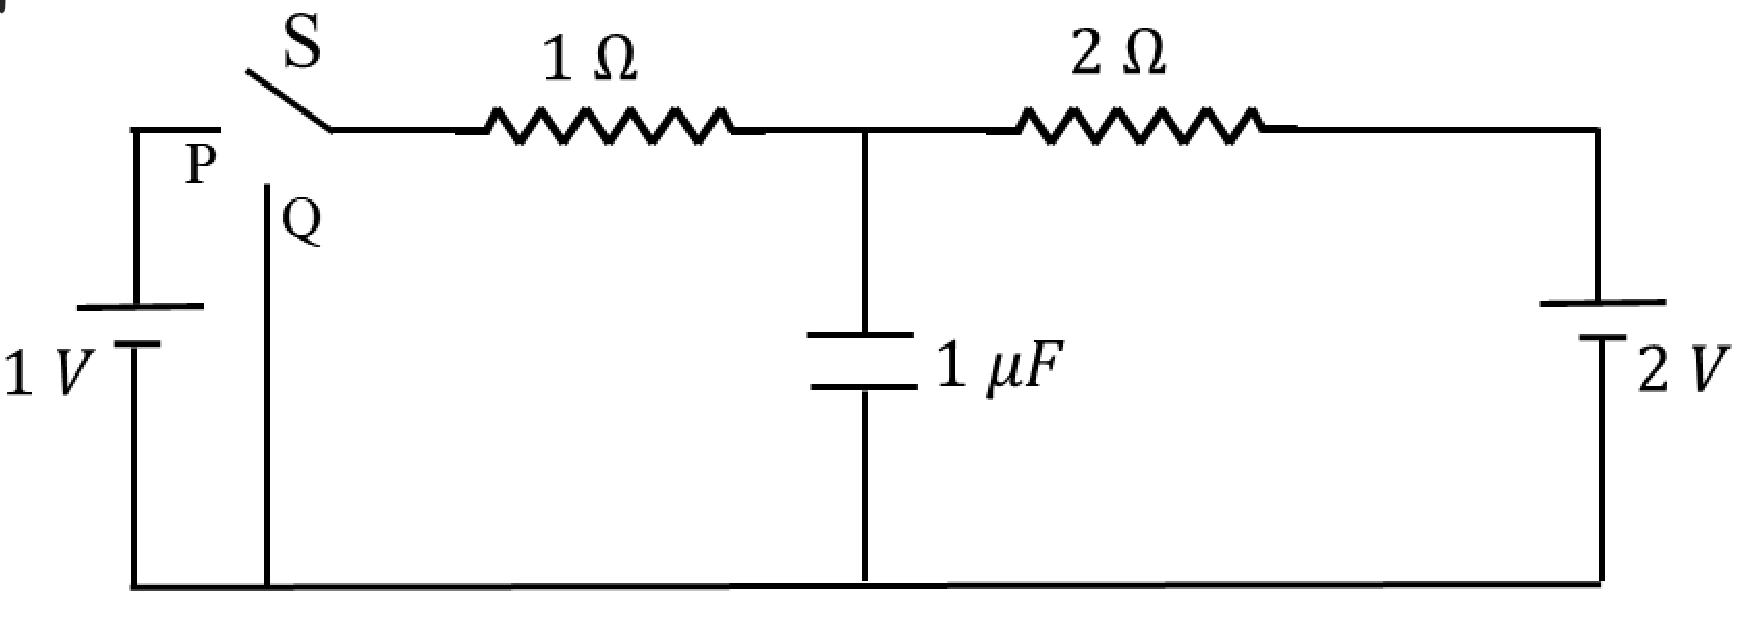
\includegraphics[width=\columnwidth]{figs/ckt.jpg}
\caption{}
\label{fig:ckt}
\end{figure}


\item Draw the circuit using latex-tikz. \\
\solution \\

\begin{circuitikz}[scale=0.9] \draw
    (0,0) to[battery1,l=1V] (0,3)
    (0,0) to[short] (1,0)
    (0,3) to[short] (0.5,3)
    node[label={above:P}] {}
    (0.5,3) to[nos, invert] (2,3)
    (1.5,3) node[label={above:S}]{}
    (1,0) to[short] (1,2.5)
    node[label={right:Q}] {}
    (1,0) to[short] (4,0)
    (2,3) to[R=$1 \ohm$] (4,3)
    node[label={above:X}]{}
    (4,0) to[C=$1 \, \mu F$] (4,3)
    (4,0) to (4,-0.2) node[ground]{}
    node[label={right:G}]{}
    (4,3) to[R=$2 \ohm$] (7,3)
    (4,0) to[short] (7,0)
    (7,0) to[battery1,l=2V] (7,3)
    ;
\end{circuitikz}

\item Find $q_1$.\\
\solution

After a long time in position $P$, the charge on the capacitor is $q_1 \, \mu C$. \\
Current through the capacitor is $0$ at steady state. So, current only flows in the outer loop.\\
Let the total current in the circuit be $I$.
\vspace{2mm}

\begin{circuitikz}[scale=1] \draw
    (0,0) to[battery1,l=1V] (0,3)
    (0,3) to[short] (1,3)
    (1,3) node[label={above:P}]{}
    (0,0) to[short] (3,0)
    (1,3) to[R=$1 \ohm$] (3,3)
    (3.4,3) node[label={above:X}]{}
    % (4,0) to[C=$1 \, \mu F$] (4,3)
    (3.5,0) to (3.5,-0.2) node[ground]{}
    (3.5,0) node[label={above:G}]{}
    (3,3) to[R=$2 \ohm$] (6,3)
    (3,0) to[short] (6,0)
    (6,0) to[battery1,l=2V,f=$I$] (6,3)
    ;
\end{circuitikz}

\begin{align}
    I &= \frac{(2 - 1) V}{(1 + 2)\ohm} \\
    I &= \frac{1}{3} A
\end{align}

Potential difference across the capacitor \brak{\text{across the points $G$ and $X$}} is 
\begin{align}
    V_{C_0} &= 2 - 2 \times \frac{1}{3} = 1.33 V \\
    q_1 &= C V_{C_0} \\
    q_1 &= 1 \mu F \times 1.33 V \\
    q_1 &= 1.33 \mu C
\end{align}
\item Show that the Laplace transform of $u(t)$ is $\frac{1}{s}$ and find the ROC. \\
\solution \\
By definition of Laplace transform of $u(t)$, we have
\begin{align}
    \mathcal{L}\{u(t)\} &= \int_{-\infty}^{\infty} u(t) e^{-st}\, dt \\
    &= \int_{0}^{\infty} e^{-st}\, dt \\
    &= \biggl(-\frac{e^{-st}}{s} \biggr) ^{+\infty}_{0} \\
    \mathcal{L}\{u(t)\} &= \frac{1}{s} 
\end{align}

$\lim_{s \to \infty} e^{-st} = 0$ only when $Re(s) > 0$. \\
The ROC is $Re(s) > 0$.

\item Show that 
\begin{align}
e^{-at}u(t) \system{L} \frac{1}{s+a}, \quad a > 0
\end{align}
and find the ROC. \\
\solution
\begin{align}
    \mathcal{L}\{e^{-at}u(t)\} &= \int_{-\infty}^{\infty} e^{-at}u(t) e^{-st}\, dt \\
    &= \int_{0}^{\infty} e^{-at} e^{-st}\, dt \\
    &= \biggl(-\frac{e^{-at}e^{-st}}{s+a} \biggr) ^{+\infty}_{0} \\
    \mathcal{L}\{e^{-at}u(t)\} &= \frac{1}{s+a}
\end{align}

$\lim_{s \to \infty} e^{-(s+a)t} = 0$ only when $Re(s) > -a$. \\
The ROC is $Re(s) > -a$.

\item Now consider the following resistive circuit transformed from 
Fig. \ref{fig:ckt}
\begin{figure}[!ht]
\centering
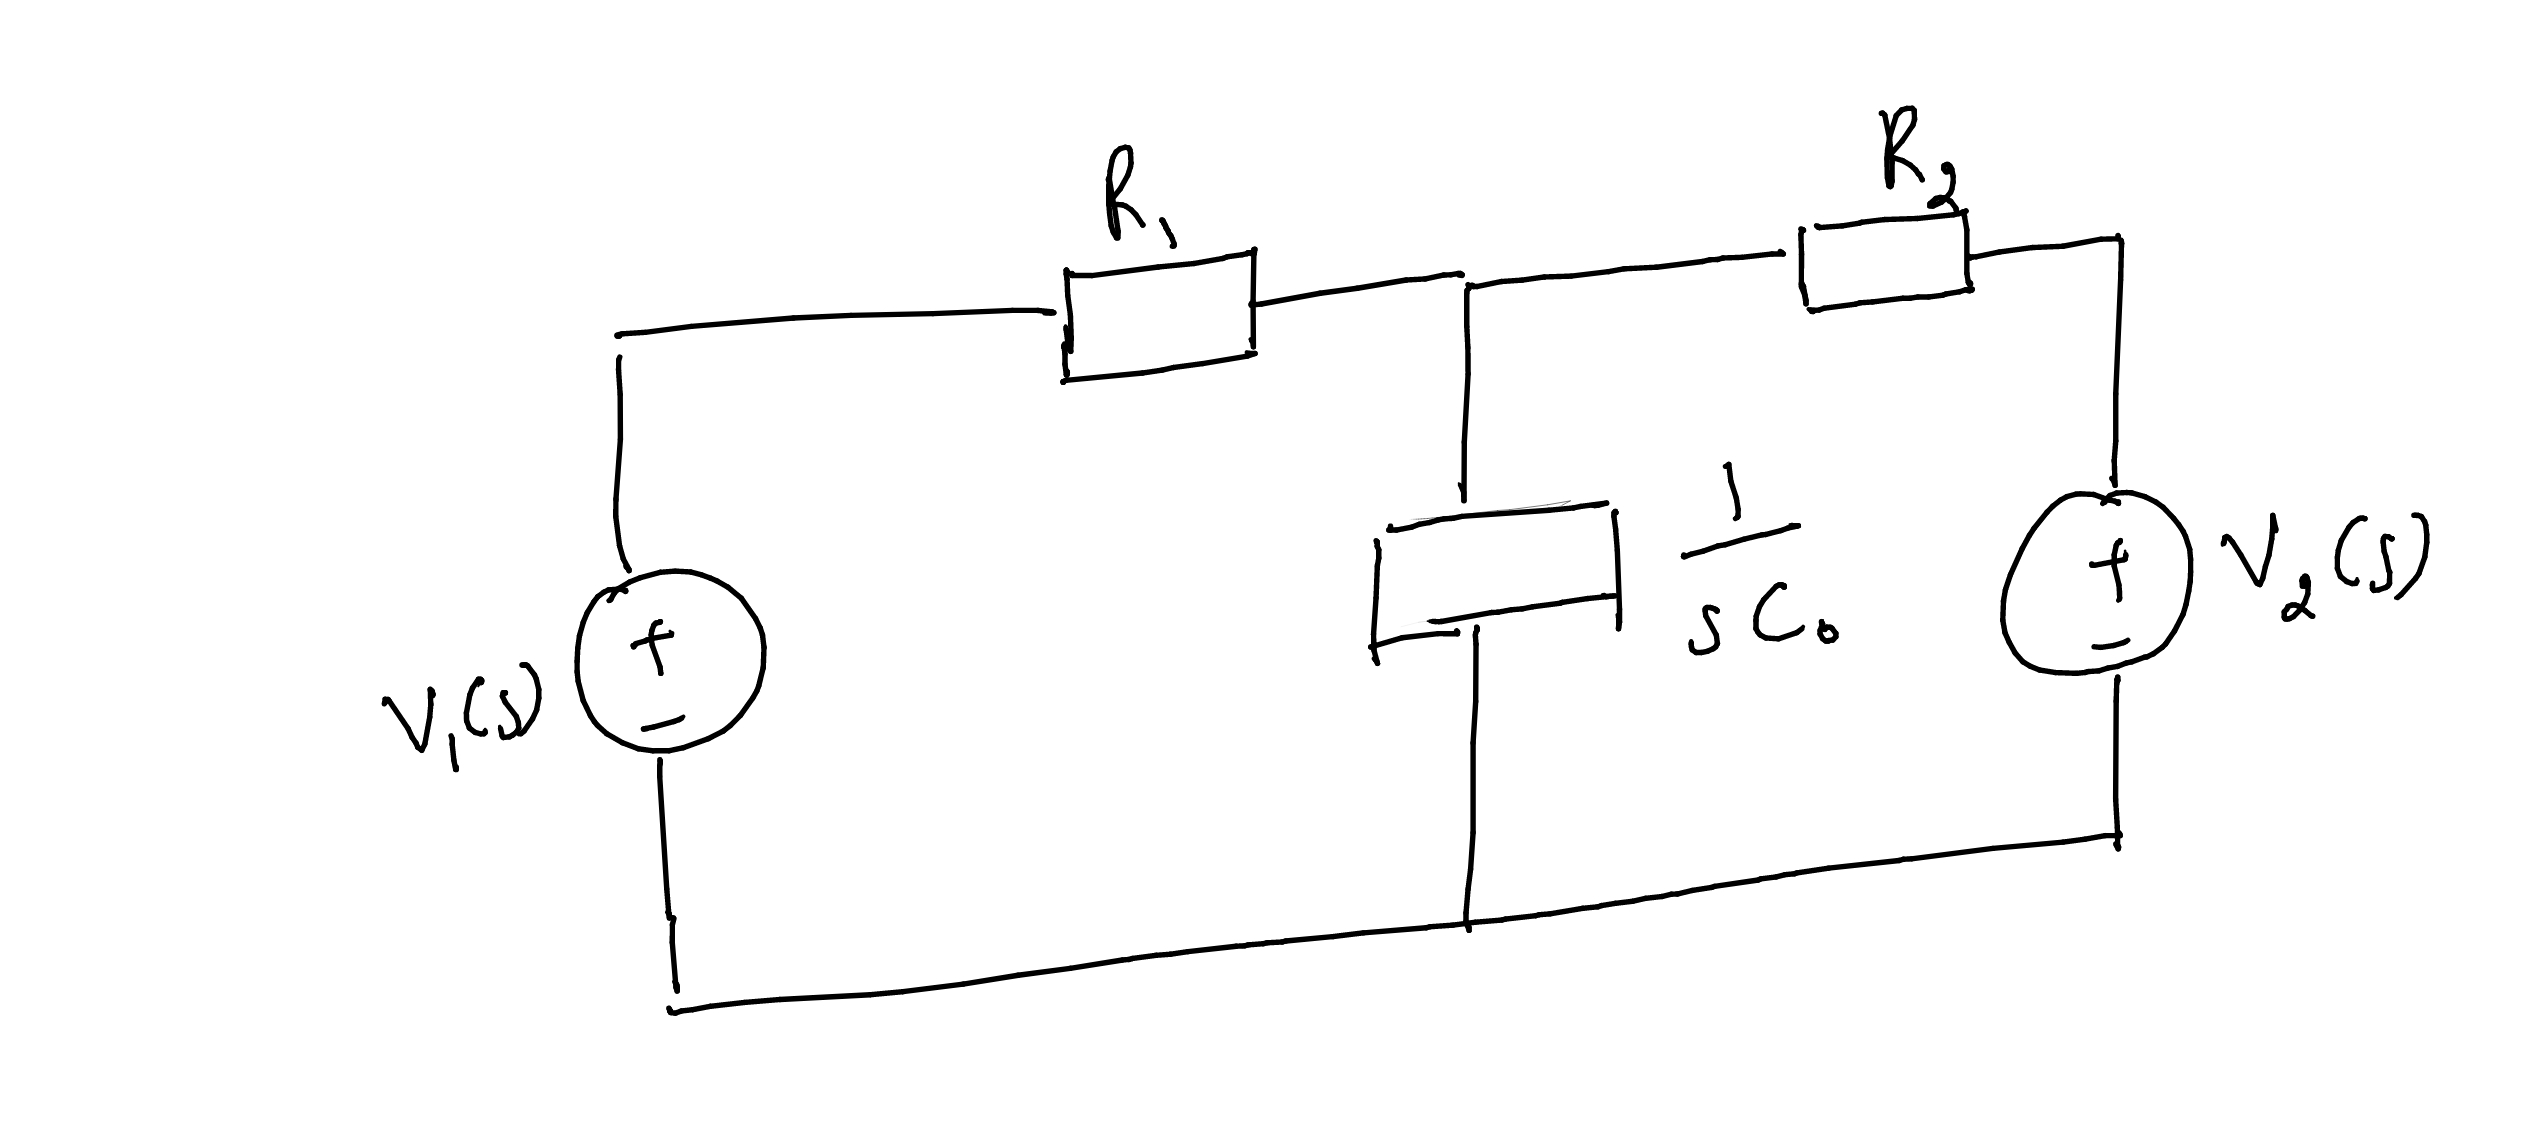
\includegraphics[width=\columnwidth]{figs/lap-ckt.jpg}
\caption{}
\label{fig:lap-ckt}
\end{figure}
where 
\begin{align}
u(t) \system{L} V_1(s)
\\
2u(t) \system{L} V_2(s)
\end{align}
Find the voltage across the capacitor $V_{C_0}(s)$.

\solution
\begin{align}
    V_1(s) &= \mathcal{L}(u(t)) = \frac{1}{s} \\
    V_2(s) &= \mathcal{L}(2u(t)) = \frac{2}{s}
\end{align}

Potential across the capacitor is $V_{C_0}(s)$ and assume that the bottom is grounded. \\
Applying Kirchoff's circuital law at the junction, we have 
\begin{align}
    &\frac{V_{C_0}(s) - V_1(s)}{R_1} + \frac{V_{C_0}(s) - V_2(s)}{R_2} + \frac{V_{C_0}(s)}{\frac{1}{s C_0}} = 0 \\
    &V_{C_0}(s) \brak{\frac{1}{R_1} + \frac{1}{R_2} + s C_0} = \frac{V_1(s)}{R_1} + \frac{V_2(s)}{R_2} \\
    &V_{C_0}(s) = \frac{V_1(s)R_2 + V_2(s)R_1}{R_1 + R_2 + s C_0 R_1 R_2} \\
    &V_{C_0}(s) = \frac{R_2 + 2R_1}{s(R_1 + R_2 + s C_0 R_1 R_2)} 
\end{align}

\item Find $v_{C_0}(t)$.  Plot using python. \\
\solution
Factoring $V_{C_0}(s)$, we have 
\begin{align}
    &V_{C_0}(s) = \frac{\brak{\frac{R_2 + 2R_1}{R_1 + R_2}}}{s} - \frac{R_1 R_2 C_0 \brak{\frac{R_2 + 2R_1}{R_1 + R_2}}}{R_1 + R_2 + sC_0 R_1 R_2} \\
    &= \brak{\frac{R_2 + 2R_1}{R_1 + R_2}} \brak{\frac{1}{s} - \frac{R_1 R_2 C_0}{R_1 + R_2 + sC_0 R_1 R_2}} \\
    &= \brak{\frac{R_2 + 2R_1}{R_1 + R_2}} \brak{\frac{1}{s} - \frac{1}{\frac{1}{R_2 C_0} + \frac{1}{R_1 C_0} + s}} 
\end{align}
Applying inverse Laplace transform on both sides, we obtain
\begin{align}
    v_{C_0}(t) = &\frac{R_2 + 2R_1}{R_1 + R_2} \brak{u(t) - e^{-\brak{\frac{1}{R_1 C_0} + \frac{1}{R_2 C_0}} \, t} u(t)}
\end{align}
Using the values $R_1 = 1 \, \Omega$, $R_2 = 2 \, \Omega$, $C_0 = 1 \, \mu F$, we have
\begin{align}
    v_{C_0}(t) = \frac{4}{3} u(t) \brak{1 - e^{-1.5 \times 10^{6} \, t}} 
\end{align}

Download the following python code for plot of $v_{C_0}(t)$. 
\begin{lstlisting}
    wget 2_7.py
\end{lstlisting}

\begin{figure}[!ht]
    \centering
    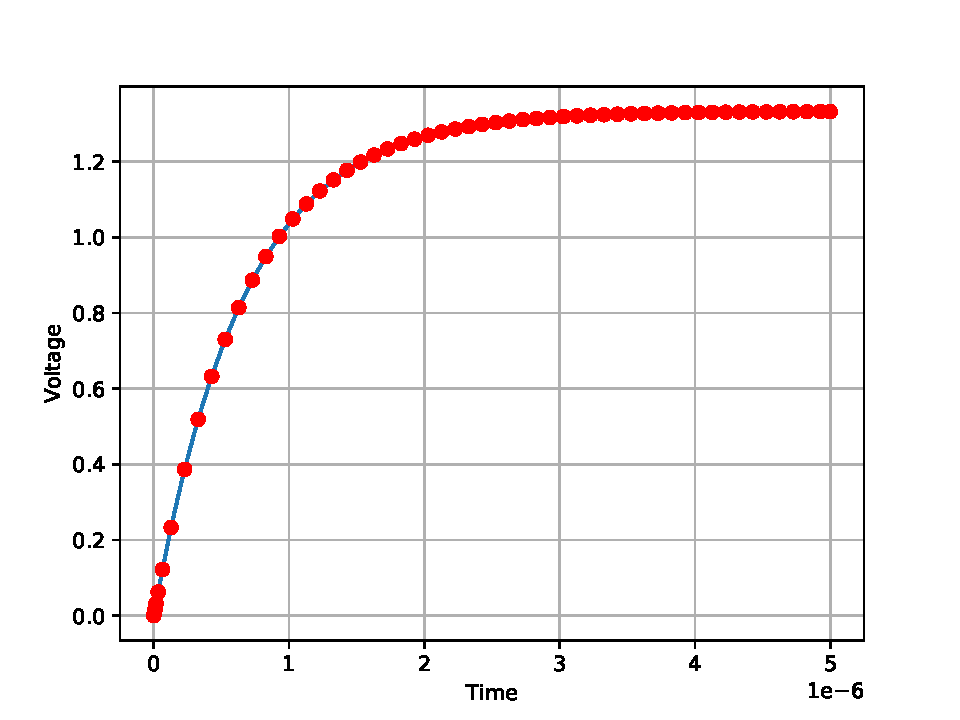
\includegraphics[width=\columnwidth]{figs/2_7.pdf}
\end{figure}
\pagebreak

\item Verify your result using ngspice.\\
\solution
Download the following code for ngspice simulation.
\begin{lstlisting}
    wget 2_8.spice
\end{lstlisting}
Run using the command 
\begin{lstlisting}
    ngspice 2_8.spice
\end{lstlisting}

The plot obtained is show below 
\begin{figure}[!hb]
    \centering
    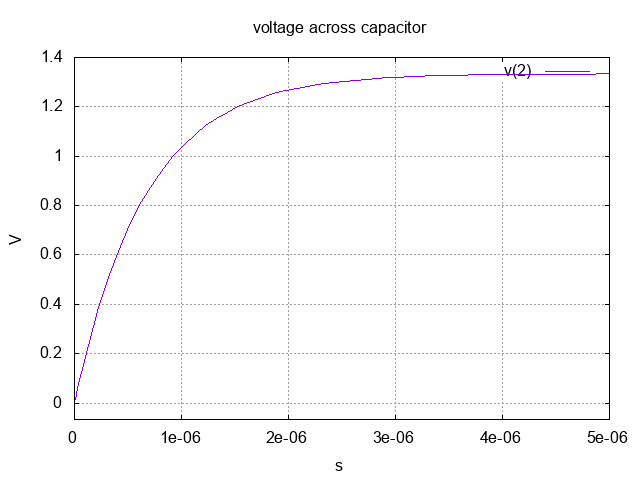
\includegraphics[width=0.9\columnwidth]{figs/2_8.png}
\end{figure}

\item Obtain Fig. 
\ref{fig:lap-ckt}
using the equivalent differential equation. 

\solution

\begin{circuitikz}[scale=0.9] \draw
    (0,0) to[battery1,l=$V_1$] (0,3)
    (0,0) to[short] (1,0)
    (0,3) node[label={above:P}] {}
    (1,0) to[short] (4,0)
    (0,3) to[R=$R_1$, -*, i<=$i_1$] (4,3)
    node[label={above:X}]{}
    (4,0) to[C=$C_0$, i<_=$i_2$] (4,3)
    (4,0) to (4,-0.2) node[ground]{}
    node[label={right:G}]{}
    (4,3) to[R=$R_2$] (7,3)
    (4,0) to[short] (7,0)
    (7,0) to[battery1,l=$V_2$, i=$i$] (7,3)   
    ;
\end{circuitikz}

Applying Kirchoff's loop law, we have 
\begin{align}
    &V_{C_0} = i_1 R_1 + V_1 \\
    &V_2 - iR_2 = V_{C_0} \\
    &V_2 - (i_1 + i_2)R_2 = V_{C_0} \\
    %&V_2 - \frac{V_{C_0} - V_1}{R_1} R_2  - i_2 R_2 = V_{C_0} \\
    &i_2 = \frac{d\brak{C_0 V_{C_0}}}{dt} 
    %&V_2 - \frac{V_{C_0} - V_1}{R_1} R_2  - \frac{d\brak{C_0 V_{C_0}}}{dt} R_2 = V_{C_0} \\
    %&V_2 + \frac{V_1 R_2}{R_1} = V_{C_0} \brak{1 + \frac{R_2}{R_1}} + R_2 C_0 \frac{d V_{C_0}}{dt} 
\end{align}

%Applying Laplace transform to this differential equation, we have 
%\begin{align}
%	&\brak{\frac{V_2}{s} + \frac{R_2}{R_1} \frac{V_1}{s}} = V_{C_0} (s) \brak{1 + \frac{R_2}{R_1} + s R_2 C_0} \\
%	&V_{C_0}(s) = \frac{R_1 V_2 + R_2 V_1}{s \brak{R_1 + R_2 + s R_1 R_2 C_0}} 
%\end{align}

To find resistance of capacitor in $s-$domain, we calculate the value of 
$\frac{V_{C_0}}{s}$

\begin{align}
	&\mathcal{L} \brak{\frac{d V_{C_0}}{dt}} = \int_{-\infty}^{\infty} \frac{d V_{C_0}}{dt} e^{-st} dt \\
	&= e^{-st} V_{C_0}(t) + \int_{-\infty}^{\infty} s e^{-st} V_{C_0}(t) dt \\
	&= s V_{C_0}(s) - V_{C_0}(0) \\
	&= s V_{C_0}(s)
\end{align}

To find resistance of capacitor in $s-$domain, we calculate the value of \\
\begin{align}
	\frac{V_{C_0}(s)}{i_2 (s)} &= \frac{V_{C_0}(s)}{s \, C_0 \, V_{C_0}(s)} \\
				&= \frac{1}{s C_0}
\end{align}

The circuit elements will be as follows
\begin{align}
	V_1(t) \overset{\mathcal{L}}{\longleftrightarrow} \frac{1}{s} \quad  V_2(t) \overset{\mathcal{L}}{\longleftrightarrow} \frac{2}{s}\\
	C_0 \overset{\mathcal{L}}{\longleftrightarrow} \frac{1}{sC_0}
\end{align}
Resistors will remain unchanged in $s-$domain
Obtained figure is depicted below 

\begin{circuitikz}[american] \draw
    (0,0) to[V, v=$V_{1} (s)$] (0,3)
    node[label={above:Q}]{}
    (0,0) to[short] (3,0)
    (0,3) to[R=$R_1$] (3,3)
    (3,0) to[cC = $\frac{1}{s C_0}$,invert] (3,3)
    (3,0) to[short] (6,0)
    (3,3) to[R=$R_2$] (6,3)
    (6,0) to[V, v=$V_{2} (s)$] (6,3)
    ;
\end{circuitikz}
\end{enumerate}
%%%%%%%%%%%%%%%%%%%%%%%%%%%%%%%%%%%%%%%%%%%%%%%%%%%%%%%%%
\section{Initial Conditions}
\begin{enumerate}[label=\arabic*.,ref=\thesection.\theenumi]
\numberwithin{equation}{section}
\item Find $q_2$ in Fig. 
\ref{fig:ckt}.\\
\solution
After a long time in position $Q$, the charge on the capacitor is $q_2 \, \mu C$. \\
Current through the capacitor is $0$ in steady state. 
So, current only flows in the outer loop.\\
Let the total current in the circuit be $I$.

\vspace{5mm}

\begin{circuitikz}[scale=1] \draw
    %(0,0) to[battery1,l=1V,invert] (0,3)
    (0,0) to[short] (0,3)
    (0.5,3) node[label={above:Q}]{}
    (0,0) to[short] (3,0)
    (0,3) to[R=$1 \ohm$] (3,3)
    (3.5,3) node[label={above:X}]{}
    % (4,0) to[C=$1 \, \mu F$] (4,3)
    (3,0) to (3,-0.2) node[ground]{}
    (3.5,0) node[label={above:G}]{}
    (3,3) to[R=$2 \ohm$] (6,3)
    (3,0) to[short] (6,0)
    (6,0) to[battery1,l=2V,f=$I$] (6,3)
    ;
\end{circuitikz}

\begin{align}
    I = \frac{2V}{(1 + 2)\ohm} = \frac{2}{3} A
\end{align}

So, the potential difference across the capacitor (across the points $G$ and $X$) is  
\begin{align}
    V_{C_0} &= 2 - \brak{\frac{2}{3} \times 2} = 0.67 V \\
    q_2 &= C V_{C_0} \\
    q_2 &= 1 \, \mu C \times 0.67 V \\  
    q_2 &= 0.67 \, \mu C 
\end{align}

\item Draw the equivalent $s$-domain resistive circuit when S is switched to position Q.  Use variables $R_1, R_2, C_0$ for the passive elements.
Use latex-tikz.
\label{prob:init}
\\ \solution 
\\ \\
\begin{circuitikz}[american] \draw
    %(0,0) to[V,invert, v=$V_{1} (s)$] (0,3)
    (0,0) to[short] (0,3)
    node[label={above:Q}]{}
    (0,0) to[short] (3,0)
    (0,3) to[R=$R_1$] (3,3)
    (3,0) to[cC = $\frac{1}{s C_0}$,invert] (3,1.5)
    (3,1.5) to[V,v=$\frac{4}{3s}$] (3,3)
    (3,0) to[short] (6,0)
    (3,3) to[R=$R_2$] (6,3)
    (6,0) to[V, v=$V_{2} (s)$] (6,3)
    ;
\end{circuitikz}

\item $V_{C_0}(s)$ = ? \\ 
\solution
\begin{align}
    &V_{C_0}(s) \brak{\frac{R_1 + R_2 + sC_0 R_1 R_2}{R_1 R_2}} = \frac{6 + 4C_0 sR_2}{3s R_2} \\
    &V_{C_0}(s) = \frac{\brak{\frac{2R_1}{s}} + \brak{\frac{4C_0}{3}} R_1 R_2}{\brak{R_1 + R_2 + sC_0 R_1 R_2}}
\end{align}

\item $v_{C_0}(t)$ = ? Plot using python. \\
\solution
Splitting into partial fractions, we have
\begin{align}
    &V_{C_0}(s) = \frac{\brak{\frac{2R_1}{s}} + \brak{\frac{4C_0}{3}} R_1 R_2}{\brak{R_1 + R_2 + sC_0 R_1 R_2}} 
\end{align}
\begin{align}
    V_{C_0}(s) = &\frac{2R_1}{s\brak{R_1 + R_2 + sC_0 R_1 R_2}} + \\
    &\frac{4C_0 R_1 R_2}{3\brak{R_1 + R_2 + sC_0 R_1 R_2}} 
\end{align}
\begin{flalign}
= \frac{2R_1}{R_1 + R_2}&\brak{\frac{1}{s} - \frac{1}{\brak{\frac{1}{R_1C_0} + \frac{1}{R_2C_0} + s}}} + \\
& \frac{4}{3 \brak{\frac{1}{R_1C_0} + \frac{1}{R_2C_0} + s}}
\end{flalign}
Applying inverse Laplace transform,
\begin{align}
    v_{C_0}(t) &= \frac{2R_1}{R_1 + R_2}\brak{1-e^{\frac{-t}{C_0}\brak{\frac{1}{R_1}+\frac{1}{R_2}}}}u(t)\nonumber\\
    &+\frac{4}{3}e^{\frac{-t}{C_0}\brak{\frac{1}{R_1}+\frac{1}{R_2}}}u(t)
\end{align}
Substituting the values, we have

\begin{align}
    v_{C_0}(t) &= \frac{2}{3}\brak{1-e^{-1.5t\times10^6}}u(t)+    \frac{4}{3}e^{-1.5t\times10^6}u(t)\\
    v_{C_0}(t) &=\frac{2}{3}\brak{1+e^{-1.5t\times10^6}}u(t)\label{eq:vct2}
\end{align}

Download the following python code for the plot
\begin{lstlisting}
    wget 3_4.py
\end{lstlisting}
\begin{figure}[!ht]
    \centering
    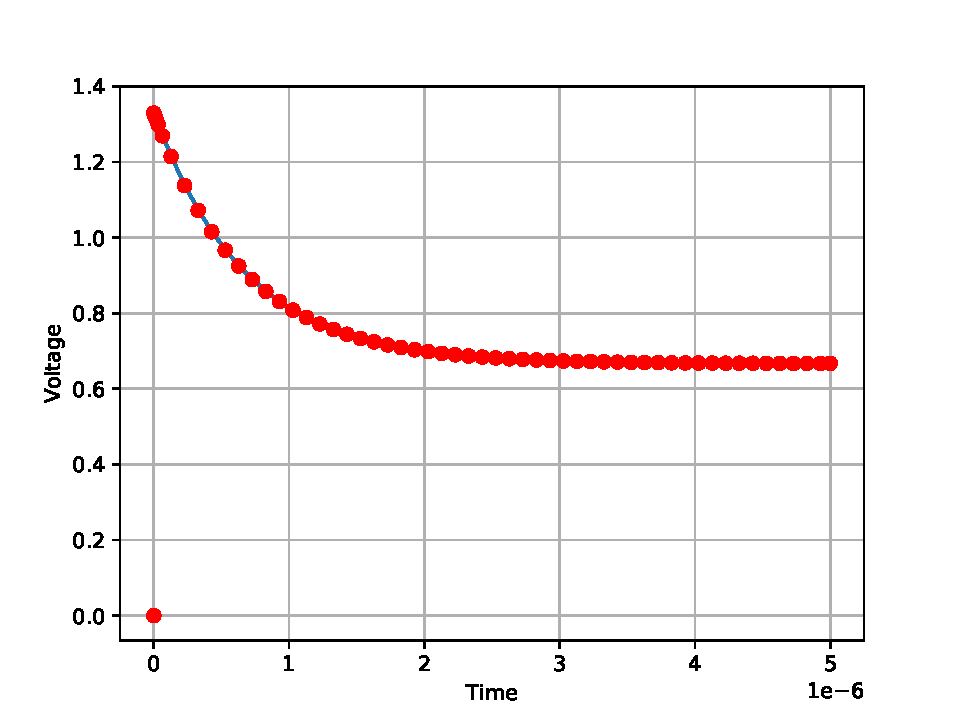
\includegraphics[width=\columnwidth]{figs/3_4.pdf}
\end{figure}
\pagebreak
\item Verify your result using ngspice.

Download the following code for ngspice simulation. 
\begin{lstlisting}
    wget 3_4.spice
\end{lstlisting}
Run using the command 
\begin{lstlisting}
    ngspice 3_4.spice
\end{lstlisting}
The plot obtained is show below 
\begin{figure}[!ht]
    \centering
    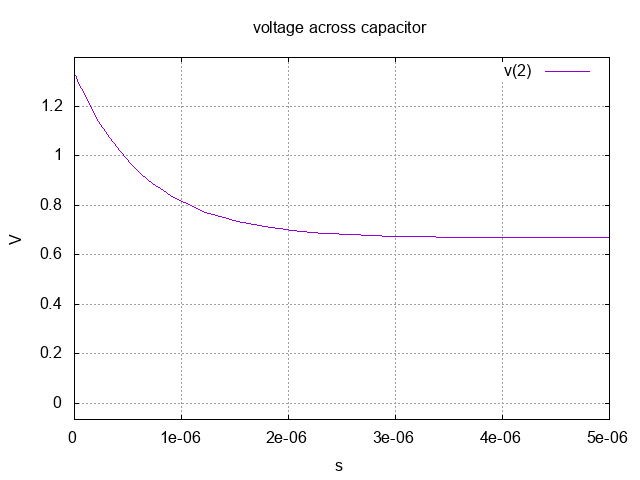
\includegraphics[width=\columnwidth]{figs/3_5.png}
\end{figure}

\item Find $v_{C_0}(0-), v_{C_0}(0+)$ and  $v_{C_0}(\infty) $. \\
\solution
At $t = 0^-$, the switch is in position $P$ for a long time 
\begin{align}
    v_{C_0}(0-) = \frac{4}{3} V
\end{align}

At $t = 0^+$, the switch has just shifted to position $Q$ 
\begin{align}
    \lim_{t -> 0^+} v_{C_0}(t) &= \lim_{t -> 0^+} \frac{2}{3}\brak{1+e^{-1.5t\times10^6}}u(t) \\
    v_{C_0}(0+) &= \frac{4}{3}V
\end{align}

At $t = \infty$, the switch is in position $Q$ for a long time
\begin{align}
   lim_{t -> \infty} v_{C_0}(t) &= \lim_{t -> \infty} \frac{2}{3}\brak{1+e^{-1.5t\times10^6}}u(t) \\
   v_{C_0}(\infty) &= \frac{2}{3}V
\end{align}

\pagebreak
\item Obtain the Fig.  in problem 
\ref{prob:init}
using the equivalent differential equation. \\
\solution

\begin{circuitikz}[scale=0.9] \draw
    (0,0) to[short] (0,3)
    (0,0) to[short] (1,0)
    (0,3) node[label={above:P}] {}
    (1,0) to[short] (4,0)
    (0,3) to[R=$R_1$, -*, i<=$i_1$] (4,3)
    node[label={above:X}]{}
    (4,0) to[C=$C_0$, i<_=$i_2$] (4,3)
    (4,0) to (4,-0.2) node[ground]{}
    node[label={right:G}]{}
    (4,3) to[R=$R_2$] (7,3)
    (4,0) to[short] (7,0)
    (7,0) to[battery1,l=$V_2$, i=$i$] (7,3)   
    ;
\end{circuitikz}

Applying Kirchoff's loop law, we have 
\begin{align}
    &V_{C_0} = i_1 R_1 \\
    &V_2 - iR_2 = V_{C_0} \\
    &V_2 - (i_1 + i_2)R_2 = V_{C_0} \\
    %&V_2 - \frac{V_{C_0} - V_1}{R_1} R_2  - i_2 R_2 = V_{C_0} \\
    &i_2 = \frac{d\brak{C_0 V_{C_0}}}{dt} 
    %&V_2 - \frac{V_{C_0} - V_1}{R_1} R_2  - \frac{d\brak{C_0 V_{C_0}}}{dt} R_2 = V_{C_0} \\
    %&V_2 + \frac{V_1 R_2}{R_1} = V_{C_0} \brak{1 + \frac{R_2}{R_1}} + R_2 C_0 \frac{d V_{C_0}}{dt} 
\end{align}

%Applying Laplace transform to this differential equation, we have 
%\begin{align}
%	&\brak{\frac{V_2}{s} + \frac{R_2}{R_1} \frac{V_1}{s}} = V_{C_0} (s) \brak{1 + \frac{R_2}{R_1} + s R_2 C_0} \\
%	&V_{C_0}(s) = \frac{R_1 V_2 + R_2 V_1}{s \brak{R_1 + R_2 + s R_1 R_2 C_0}} 
%\end{align}

To find resistance of capacitor in $s-$domain, we calculate the value of 
$\frac{V_{C_0}}{s}$

\begin{align}
	&\mathcal{L} \brak{\frac{d V_{C_0}}{dt}} = \int_{-\infty}^{\infty} \frac{d V_{C_0}}{dt} e^{-st} dt \\
	&= e^{-st} V_{C_0}(t) + \int_{-\infty}^{\infty} s e^{-st} V_{C_0}(t) dt \\
	&= s V_{C_0}(s) - V_{C_0}(0) \\
	&= s V_{C_0}(s) - \frac{4}{3}  
\end{align}

% To find resistance of capacitor in $s-$domain, we calculate the value of \\
% \begin{align}
% 	\frac{V_{C_0}(s)}{i_2 (s)} &= \frac{V_{C_0}(s)}{s \, C_0 \, V_{C_0}(s)} \\
% 				&= \frac{1}{s C_0}
% \end{align}

The circuit elements will be as follows
\begin{align}
	V_1(t) \overset{\mathcal{L}}{\longleftrightarrow} \frac{1}{s} \quad  V_2(t) \overset{\mathcal{L}}{\longleftrightarrow} \frac{2}{s}\\
	C_0 \overset{\mathcal{L}}{\longleftrightarrow} \frac{1}{sC_0} \quad
    V_{C_0}(0^-) \overset{\mathcal{L}}{\longleftrightarrow} \frac{4}{3s}
\end{align}
Resistors will remain unchanged in $s-$domain
Obtained figure is depicted below 

\begin{circuitikz}[american] \draw
    (0,0) to[V, v=$V_{1} (s)$] (0,3)
    node[label={above:Q}]{}
    (0,0) to[short] (3,0)
    (0,3) to[R=$R_1$] (3,3)
    (3,0) to[cC = $\frac{1}{s C_0}$,invert] (3,1.5)
    (3, 1.5) to[V, v = $\frac{4}{3s}$] (3, 3)
    (3,0) to[short] (6,0)
    (3,3) to[R=$R_2$] (6,3)
    (6,0) to[V, v=$V_{2} (s)$] (6,3)
    ;
\end{circuitikz}
\end{enumerate}

\section{Bilinear Transform}
\begin{enumerate}[label=\arabic*.,ref=\thesection.\theenumi]
\numberwithin{equation}{section}

\item In Fig. 
\ref{fig:ckt},
Consider the case when $S$ is switched to $Q$ right in the beginning. Formulate the differential equation. \\
\solution

The circuit for the case is shown below, 
\begin{circuitikz}[scale=0.9] \draw
    (0,0) to[short] (0,3)
    node[label={above:Q}] {}
    (0,3) to[short] (1.5,3)
    (0,0) to[short] (4,0)
    (1,3) to[R=$1 \ohm$, i<=$i_1$] (4,3)
    node[label={above:X}]{}
    (4,0) to[C=$1 \, \mu F$, i<= $i_2$] (4,3)
    (4,0) to (4,-0.2) node[ground]{}
    node[label={right:G}]{}
    (4,3) to[R=$2 \ohm$] (7,3)
    (4,0) to[short] (7,0)
    (7,0) to[battery1,l=2V,i=$i$] (7,3)
    ;
\end{circuitikz}

The differential equation can be formulated as follows, 
\begin{align}
	&i_1 (R_1) = \int_{0}^{t} \frac{i_2(t)}{C_0} dt \\
	&V_2 - i R_2 - \int_{0}^{t} \frac{i_2(t)}{C_0} dt = 0 \\
	&V_2 - (i_1 + i_2) R_2 = \int_{0}^{t} \frac{i_2(t)}{C_0} dt \\
	&V_2 - (i_2 R_2) = \brak{\frac{R_2}{R_1} + 1} \int_{0}^{t} \frac{i_2(t)}{C_0} dt 	
\end{align}

Expressing the differential equation in terms of $V_{C_0}$, we have 
\begin{align}
	&V_{C_0} = \int_{0}^{t} \frac{i_2(t)}{C_0} dt\\
	&\frac{d V_{C_0}}{dt} = \frac{i_2 (t)}{C_0} \\
	&V_2 - R_2 \, C_0 \frac{d V_{C_0}}{dt} = \brak{\frac{R_1 + R_2}{R_1}} V_{C_0} \\
	& R_2 C_0 \frac{d V_{C_0}}{dt} + \brak{\frac{R_1 + R_2}{R_1}} V_{C_0} - V_2 = 0
\end{align}

\item Find $H(s)$ considering the output voltage at the capacitor. \\
\solution

Applying Laplace transform on both sides of the equation, 
\begin{align}
	&R_2 C_0 s V_{C_0}(s) + \frac{R_1 + R_2}{R_1} V_{C_0}(s) - V_2(s) = 0 \\
	&\frac{V_2(s)}{V_{C_0}(s)} =s R_2 C_0 + 1 + \frac{R_2}{R_1}
\end{align}
By definition of transfer function, we have 
\begin{align}
	&H(s) = \frac{V_{C_0}(s)}{V_2(s)} = \frac{1}{s R_2 C_0 + 1 + \frac{R_2}{R_1}}
	\label{eq:H_s}
\end{align}

On substituting the values, we get
\begin{equation}
	H(s) = \frac{5 \times 10^5}{s + 1.5 \times 10^6}
\end{equation}


\item Plot $H(s)$.  What kind of filter is it? \\

\solution Download the following Python code that plots Fig. \ref{fig-4.3}
\begin{lstlisting}
	wget 4_3.py
\end{lstlisting}

\begin{figure}[!ht]
\centering
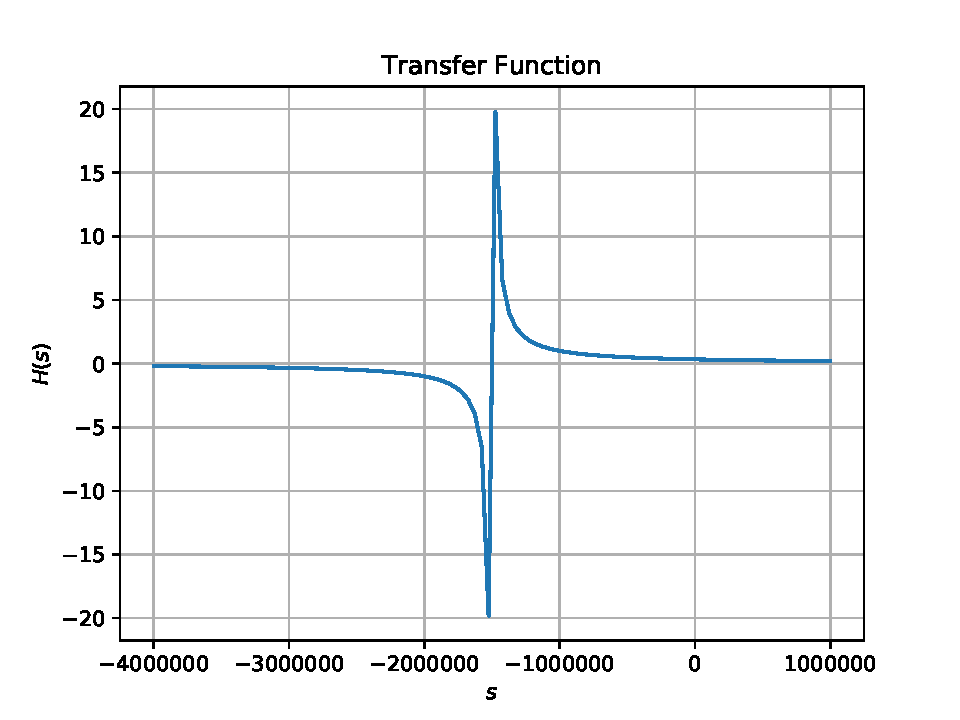
\includegraphics[width=\columnwidth]{./figs/4_3.pdf}
\caption{Plot of $H(s)$}
\label{fig-4.3}	
\end{figure}

Consider the frequency-domain transfer function by putting $s = j\omega$
\begin{align}
	&H(j\omega) = \frac{5 \times 10^5}{j\omega + 1.5 \times 10^6} \\
	&\abs{H(j\omega)} = \frac{5 \times 10^5}{\sqrt{\omega^2 + 2.25\times10^{12}}}
\end{align}
	
Since maximum value of transfer function occurs when $\omega = 0$, we have the following relation, \\
$H(j\omega)$ decreases as $\omega$ increases. \\
So, frequency ranges from $0$ to cut-off frequency. \\
Hence, the given filter is a low-pass filter. 

\item Using trapezoidal rule for integration, formulate the difference equation by considering 
\begin{align}
	y(n) = y(t)\vert_{t=n}
\end{align}

\solution
\begin{align}
	& R_2 C_0 \frac{d V_{C_0}}{dt} + \brak{\frac{R_1 + R_2}{R_1}} V_{C_0} - V_2 = 0 \\
	&C_0\frac{d V_{C_0}}{dt} = \frac{2V_2 -V_{C_0}(t)}{R_2} - \frac{V_{C_0}(t)}{R_1} \\
 & V_{C_0}(t)^{n+1}_{n} = \int_{n}^{n+1} \brak{\frac{2V_2(t) -V_{C_0}(t)}{R_2C_0} - \frac{V_{C_0}(t)}{R_1C_0}} dt
\end{align}
	
By the trapezoidal rule of integration, we approximate the following integral
\begin{align}
	\int_a^b f(t) dt = \frac{b-a}{2} \, \biggl( f(a) + f(b) \biggr)
\end{align}
	
Consider $y(t) = V_{C_0}(t)$, and simplifying using trapezoid rule on right hand side of the equation, we have 
\begin{multline}
	y(n+1) - y(n) = \frac{1}{R_2C_0}\brak{u(n)+u(n+1)} \\
	- \frac12(y(n+1) + y(n))\brak{\frac{1}{R_1C_0} + \frac{1}{R_2C_0}}
\end{multline}
	
Thus, the difference equation is
\begin{align}
\begin{split}
	&y(n+1) \brak{1 + \frac{1}{2R_1C_0} + \frac{1}{2R_2C_0}} \\= &y(n) \brak{1 - \frac{1}{2R_1C_0} - \frac{1}{2R_2C_0}} \\+ &\frac{1}{R_2C_0}\brak{u(n)+u(n+1)}
\end{split}
\label{eq:diff_eq}
\end{align}


\item Find $H(z)$. \\
\solution
Applying $\mathcal{Z}$-transform to the \eqref{eq:diff_eq} on both sides, we have 
\begin{align}
\begin{split}
	&z Y(z) \brak{\frac{2R_1 R_2 C_0 + R_1 + R_2}{2 R_1 R_2 C_0}} = \\ &Y(z) \brak{\frac{2 R_1 R_2 C_0 - R_1 - R_2}{2 R_1 R_2 C_0}} + \\ &\frac{1}{R_2 C_0} \brak{\frac{1}{1 - z^{-1}} + \frac{z}{1 - z^{-1}}}
\end{split}
\end{align}
\begin{align}
	&Y(z) = \cfrac{\brak{\cfrac{1 + z}{R_2 C_0 (1 - z^{-1})}} 2 R_1 R_2 C_0}{(2R_1 R_2 C_0 (z-1)) + (z+1)(R_1 + R_2)} \label{eq:Y_z} \\
	&X(z) = \mathcal{Z}[x(n)] = \mathcal{Z}[2 u(n)] = \frac{2}{1 - z^{-1}}
\end{align}
Using $H(z) = \frac{Y(z)}{X(z)}$, and substituting values
\begin{align}
	&H(z) = \cfrac{\brak{1 + z}}{(4 C_0 (z - 1)) + 3(z+1)}
\end{align}
\begin{align}
	&H(z) = \cfrac{1 + z^{-1}}{\brak{3 + 4 C_0} + \brak{3 - 4 C_0} z^{-1}} 
	\label{eq:H_z}
\end{align}
Region of convergence (ROC) for the $\mathcal{Z}$-transform is 
\begin{align}
	\abs{z} > \text{max} \, \Biggl( 1, \abs{\frac{3 + 4 \times 10^{-6}}{4 \times 10^{-6} - 3}} \, \Biggr) 
\end{align}
		

\item How can you obtain $H(z)$ from $H(s)$? \\
\solution
To convert $H(z)$ to $H(s)$, we use the bilinear transform. \\ It maps transfer function of $\mathcal{Z}$-transform to transfer function of $s$-domain. 
\begin{align}
	s \longleftrightarrow \frac{2}{T} \frac{1 - z^{-1}}{1 + z^{-1}}
\end{align}

$T = 1$ is the step size in trapezoidal rule

From \eqref{eq:H_s}, we have 
\begin{align}
	&H(s) = \frac{1}{s R_2 C_0 + 1 + \frac{R_2}{R_1}} \\
	&H(z) = \frac{1}{\biggl(\cfrac{1 - z^{-1}}{1 + z^{-1}} \biggr) \, 2 R_2 C_0 + 1 + \cfrac{R_2}{R_1}} \\
	&H(z) = \cfrac{1 + z^{-1}}{4 C_0 \brak{1 - z^{-1}} + 3 \brak{1 + z^{-1}}} \\
	&H(z) = \cfrac{1 + z^{-1}}{\brak{3 + 4C_0} + \brak{3 - 4 C_0}z^{-1}}
\end{align}
The equation obtained is the same as the equation \eqref{eq:H_z}.


\item Plot y(n), y(t), and voltage through ngspice. Verify that they are the same. \\
\solution
To obtain $y(n)$ from $Y(z)$, we apply inverse $\mathcal{Z}$-transform to \eqref{eq:Y_z} and substitute values.
\begin{align}
	&Y(z) = \cfrac{\brak{\cfrac{1 + z}{(1 - z^{-1})}} 2 R_1}{(2R_1 R_2 C_0 (z-1)) + (z+1)(R_1 + R_2)} \\
	&Y(z) = \cfrac{2(1+z)}{4 C_0 (1 - z^{-1})(z - 1) + 3 (1 + z)(1 - z^{-1})} 
\end{align}
\begin{align}
	&Y(z) = \cfrac{2(1+z)}{4 C_0 (z + z^{-1} - 2) + 3 (z - z^{-1})}  \\
	&= \frac{2}{3} \brak{\frac{1}{1 - z^{-1}} - \frac{4 C_0}{(4C_0 + 3) + (3 - 4C_0)z^{-1}}} \\
	&y(n) = \frac{2}{3} \biggl( 1 - \frac{\brak{1 - 7.5 \times 10^5}^n}{\brak{1 + 7.5 \times 10^5}^{n+1}} \biggr) u(n)
\end{align}
Using binomial approximation because $n \approx 10^{-7}$,   
\begin{align}
	&y(n) = \frac{2}{3} \biggl( 1 - \frac{\brak{1 - 7.5 \times 10^5}n}{\brak{1 + 7.5 \times 10^5}{n}} \biggr) u(n) 
\end{align}
Download the following python code to verify the plots of $y(t)$, ngspice plot and $y(n) = y(t) |_{t = n}$
\begin{lstlisting}
	wget 4_7.py
\end{lstlisting}

\begin{figure}[!ht]
\centering
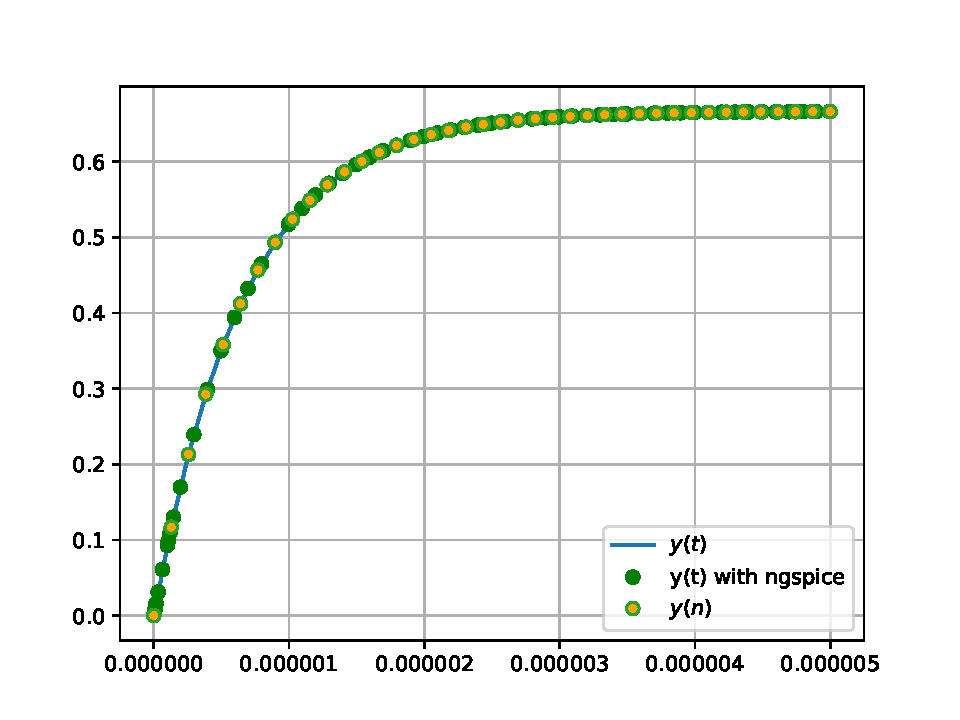
\includegraphics[width=1.0\columnwidth]{./figs/4_7.pdf}
\label{fig-4.7}	
\end{figure}
\end{enumerate}
\end{document}



